\chapter{Lab 1 Results: Why Context and Gating Matter}\label{app:lab1}

This appendix presents the experimental results from Lab~1, which tests the claims of Chapter~1: static embeddings collapse word senses, vanilla RNNs struggle with long-range dependencies, LSTMs stabilize gradients, GRUs approximate LSTMs with lower overhead, and attention reduces the Seq2Seq bottleneck.

\textbf{Task:} Char-level language modeling on Tiny Shakespeare (Experiments~1 and~3); synthetic delayed-memory probe (Experiment~2); sequence reversal (Experiment~4).

%----------------------------------------------------------------------
\section{Experiment 0: Static Embedding Polysemy Probe}

\textbf{Question:} Do static embedding vectors collapse multiple word senses into a single point?

\textbf{Setup:} GloVe 6B 100d embeddings. Query nearest neighbors for three polysemous words.

\textbf{Results:}

\begin{center}
\begin{tabular}{llcl}
\toprule
\textbf{Word} & \textbf{Top Neighbors} & \textbf{Dominant Sense} & \textbf{Minority Sense Visible?} \\
\midrule
\texttt{bank} & banks, banking, credit, investment & financial & No (0/10 river) \\
\texttt{cell} & cells, cellular, brain, tissue, phones & biology & Yes (2/10 phone) \\
\texttt{spring} & summer, autumn, winter & season & No (0/10 mechanical) \\
\bottomrule
\end{tabular}
\end{center}

\textbf{Analogy test:} Vector arithmetic still captures regular relations: \texttt{king $-$ man $+$ woman} $\to$ \texttt{queen} (cosine 0.78), \texttt{berlin $-$ paris $+$ france} $\to$ \texttt{germany} (0.89).

\begin{figure}[h]
\centering
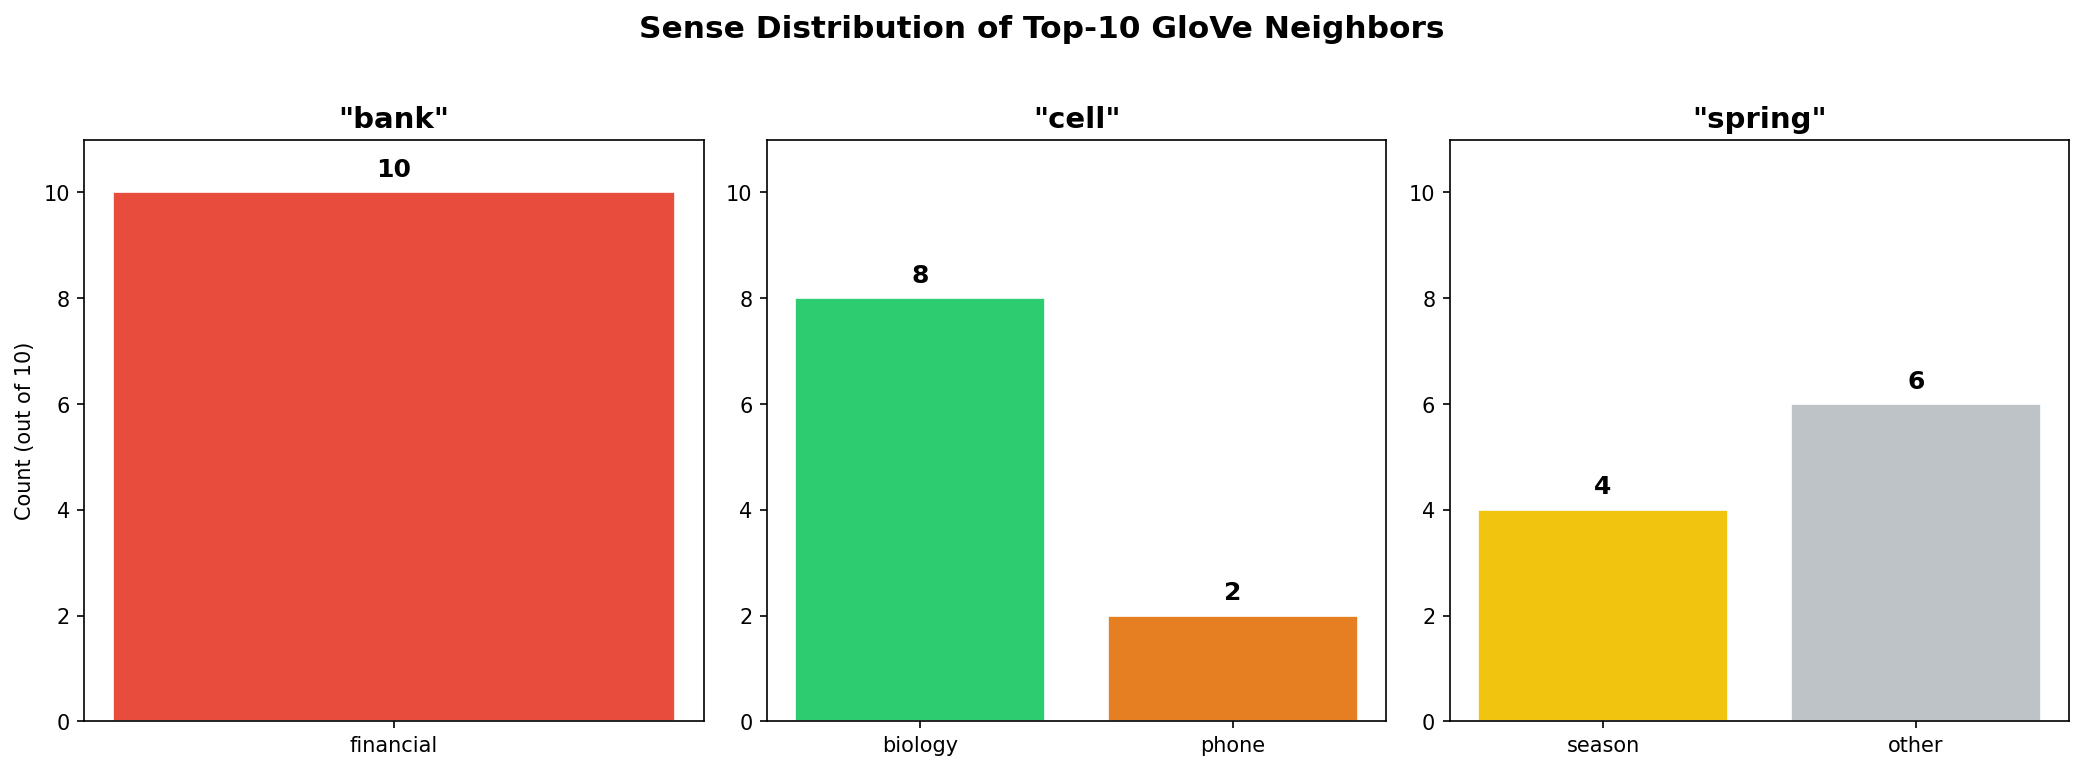
\includegraphics[width=0.65\textwidth]{labs/ch01/answers/figures/sense_distribution.png}
\caption{Sense composition of top-10 neighbors. \texttt{bank} is 100\% financial; \texttt{cell} shows biology/phone mixing; \texttt{spring} is dominated by the season sense.}
\label{fig:app-lab1-sense}
\end{figure}

\begin{figure}[h]
\centering
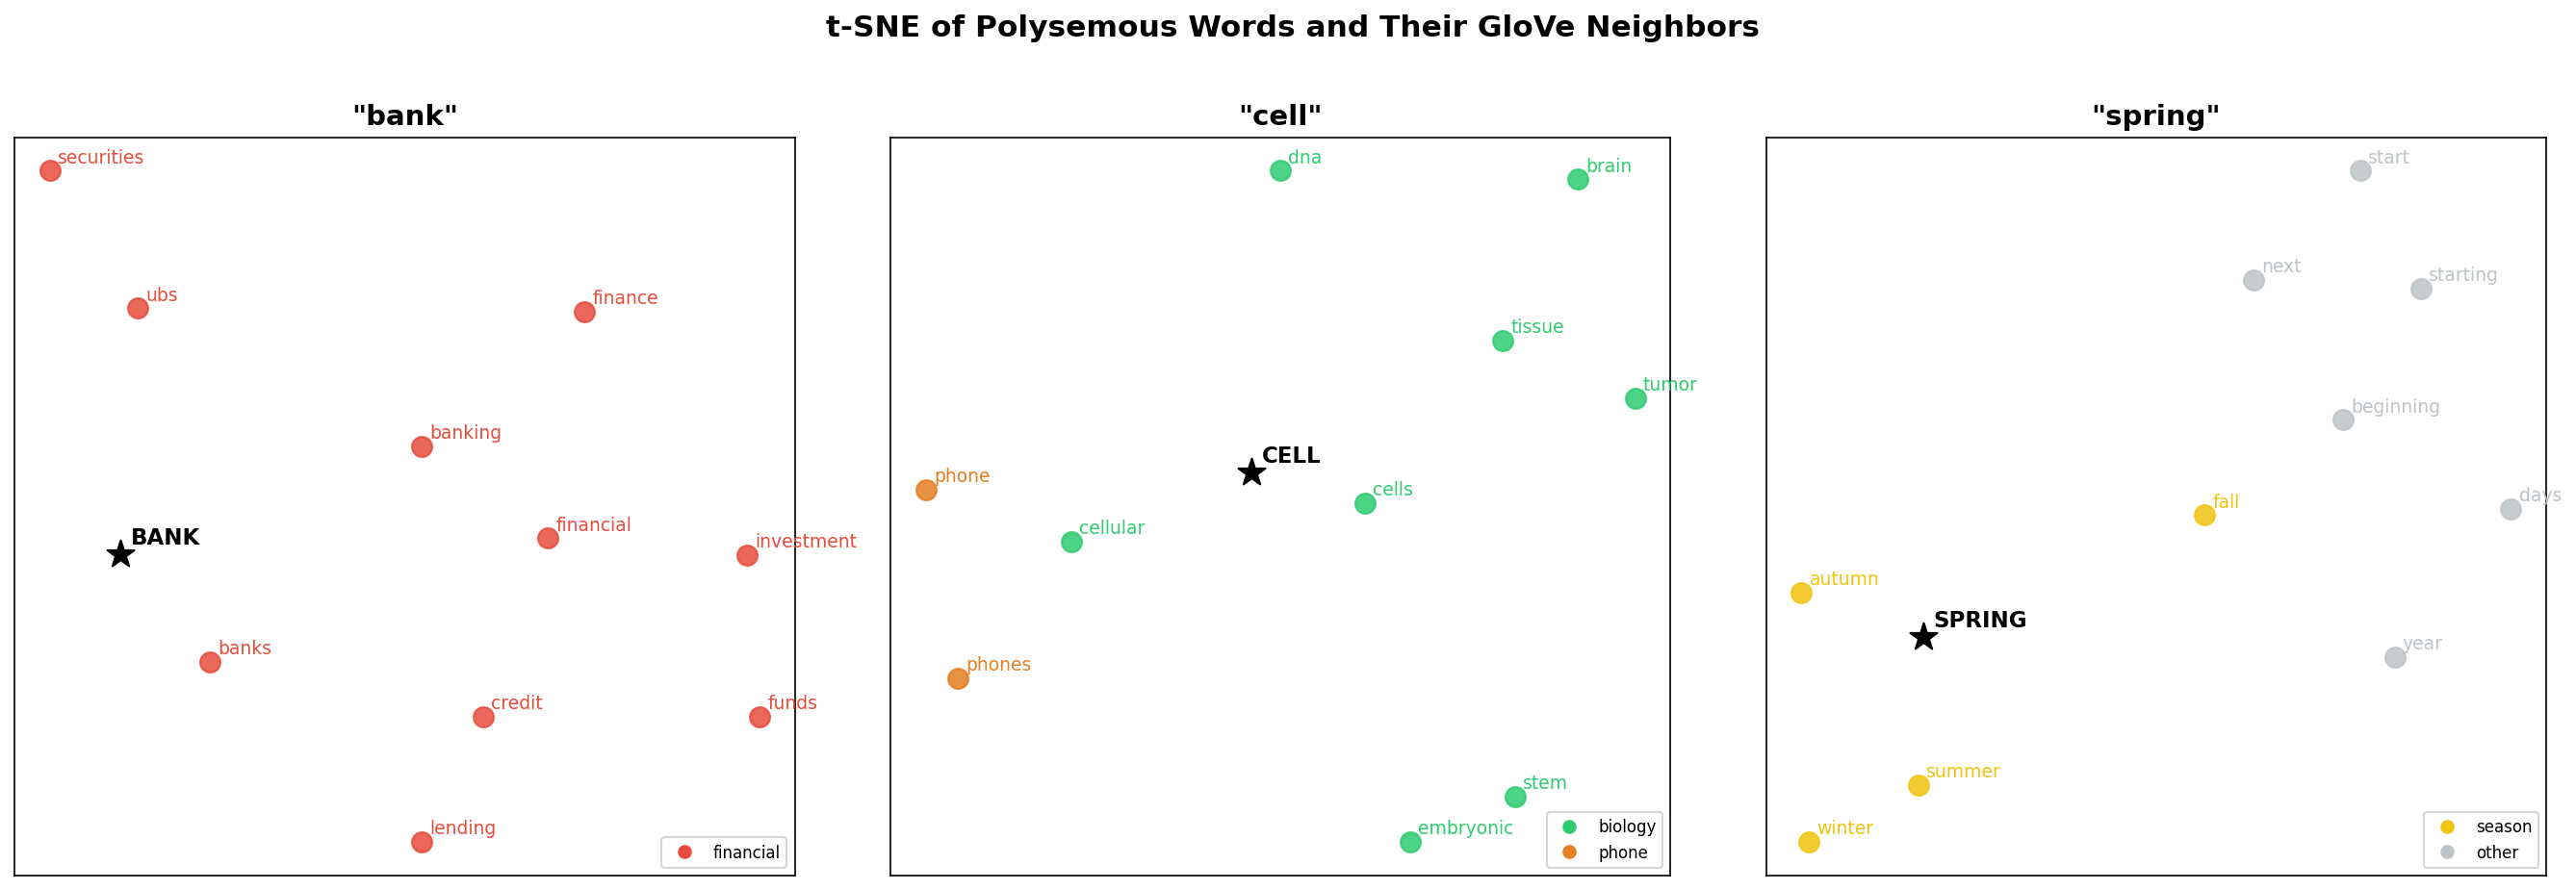
\includegraphics[width=0.7\textwidth]{labs/ch01/answers/figures/polysemy_tsne.png}
\caption{t-SNE projection of polysemous words and their neighbors. Only \texttt{cell} exhibits visible sense separation.}
\label{fig:app-lab1-tsne}
\end{figure}

\textbf{Diagnosis:} GloVe captures useful semantic structure (analogies work), but each word occupies a single point---the weighted average of all its contexts. When one sense dominates the corpus, minority senses become invisible in neighbor space.

\textbf{Core insight:} This is not merely a failure of training---it is a \emph{structural} limitation. A type-level embedding assigns one vector per word form regardless of context. More data can move that point or make the average more representative, but it cannot create separate context-dependent locations for \texttt{river bank} and \texttt{investment bank}. The solution requires \emph{token-level} representations that vary with context---exactly what RNNs and later Transformers provide. This experiment establishes the floor from which the rest of Ch1 builds upward.

%----------------------------------------------------------------------
\section{Experiment 1: Gradient Pathology}

\textbf{Question:} Does vanilla RNN exhibit gradient explosion/vanishing, and do gates solve it?

\textbf{Setup:} Train RNN/LSTM/GRU on Tiny Shakespeare (hidden=256, seq\_len=128). Two conditions: (1) normal training with gradient clipping; (2) stress test with SGD lr=1.0, no clipping.

\textbf{Results:}

\begin{center}
\begin{tabular}{lccc}
\toprule
 & \textbf{RNN} & \textbf{LSTM} & \textbf{GRU} \\
\midrule
Normal: mean grad norm & 0.344 & 0.269 & 0.260 \\
SGD stress: max grad norm & 60,241 & 0.591 & 1.788 \\
SGD stress: stable? & No (explodes) & Yes & Yes \\
\bottomrule
\end{tabular}
\end{center}

\begin{figure}[h]
\centering
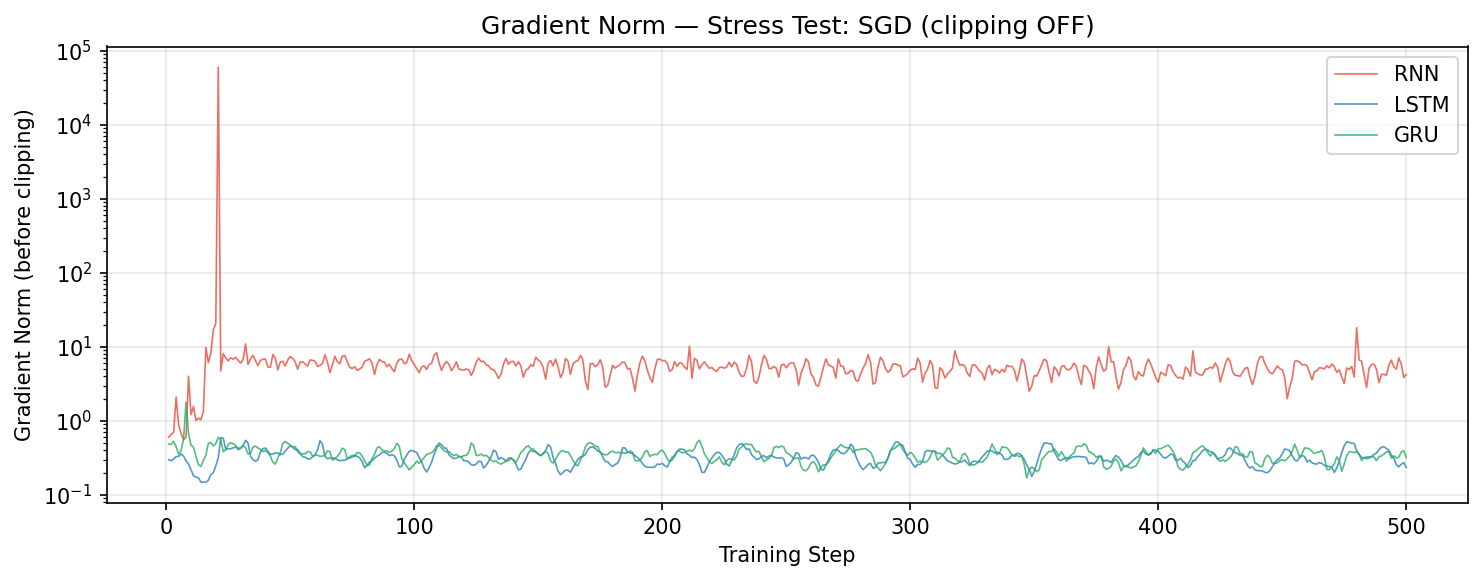
\includegraphics[width=0.7\textwidth]{labs/ch01/answers/figures/gradient_norm_stress_sgd.png}
\caption{SGD stress test: RNN gradient norm spikes to $>$60,000; LSTM and GRU remain below 2.0.}
\label{fig:app-lab1-grad}
\end{figure}

\textbf{Note:} Adam's adaptive scaling masks the pathology---the stress test must use SGD to reveal classical gradient explosion. This is an important negative result: optimizer choice affects what the experiment reveals.

\textbf{Diagnosis:} Vanilla RNNs multiply through the same recurrent weight at each step, causing exponential gradient growth or decay. LSTM cell state and GRU update gates create additive gradient highways that bypass this multiplicative chain.

\textbf{Core insight:} The gradient norm ratio tells the full story---RNN peaks at 60,241$\times$ the LSTM value. This is not a marginal instability; it is a qualitative regime change. In practice, gradient clipping ``hides'' this problem by capping the norm, but it does so by \emph{discarding information}: when a gradient is clipped, the model receives a truncated learning signal. Gates do not discard information---they \emph{route} it. This distinction (clipping as lossy workaround vs.\ gating as principled solution) is why LSTMs dominated sequence modeling for a decade. The same principle reappears in Ch3: residual connections provide the same additive highway for Transformers.

%----------------------------------------------------------------------
\section{Experiment 2: Distance Probe (Delayed Memory)}

\textbf{Question:} Can each model retain a signal over increasing distances?

\textbf{Setup:} Synthetic delayed-memory task. A signal token appears at position 0; the model must classify it after a delay of $N$ distractor tokens. Train separate models per distance $N \in \{8, 32, 128, 256\}$.

\textbf{Results:}

\begin{center}
\begin{tabular}{lcccc}
\toprule
 & $N=8$ & $N=32$ & $N=128$ & $N=256$ \\
\midrule
RNN & 100.0\% & 56.0\% & 35.9\% & 26.0\% \\
LSTM & 100.0\% & 98.8\% & 99.4\% & 99.2\% \\
GRU & 100.0\% & 99.5\% & 99.4\% & 99.4\% \\
\bottomrule
\end{tabular}
\end{center}

\begin{figure}[h]
\centering
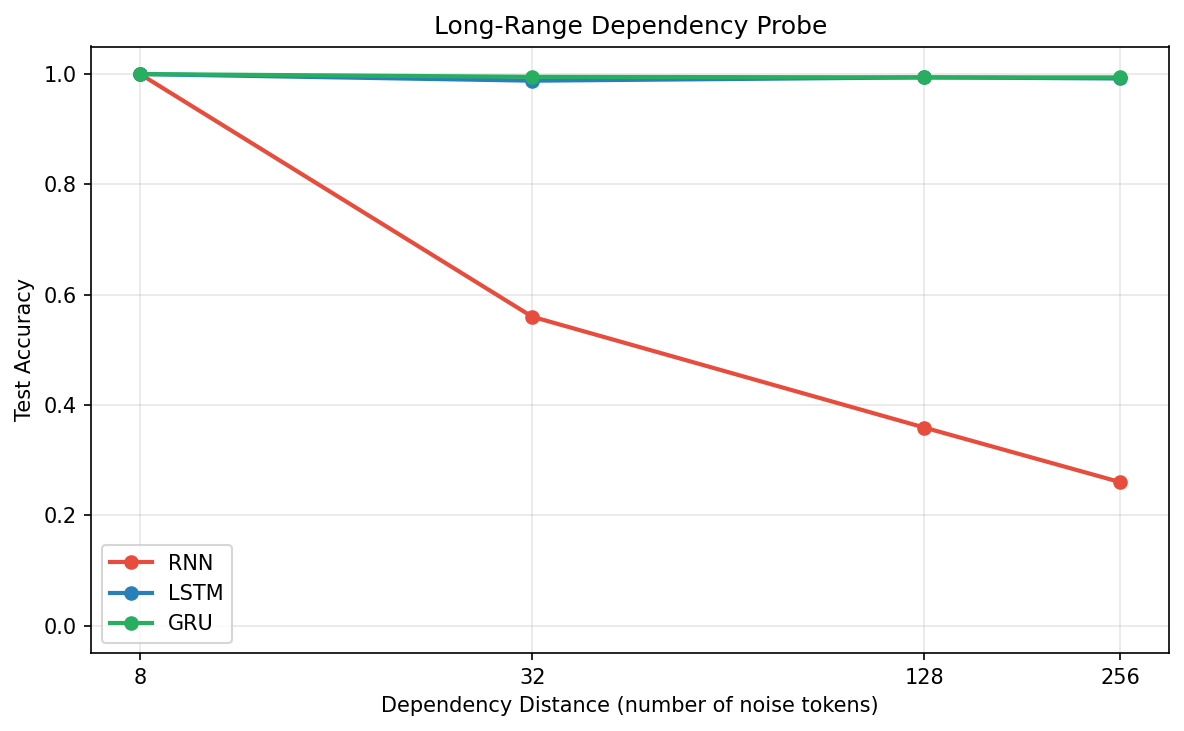
\includegraphics[width=0.65\textwidth]{labs/ch01/answers/figures/distance_probe.png}
\caption{Accuracy vs.\ dependency distance. RNN degrades sharply; LSTM and GRU maintain near-perfect accuracy at all distances.}
\label{fig:app-lab1-distance}
\end{figure}

\textbf{Diagnosis:} The RNN's accuracy at $N=256$ (26\%) is near random for 10 classes, confirming that the signal is lost. LSTM and GRU cell state / update gates allow selective preservation of information across arbitrary distances.

\textbf{Core insight:} This experiment separates two confounded claims: (1) RNNs cannot \emph{propagate gradients} over long distances (Exp~1), and (2) RNNs cannot \emph{store information} over long distances (this experiment). Both are true, but they are distinct failure modes. Exp~1 shows the model cannot \emph{learn} from distant signals; Exp~2 shows that even if it could learn, it cannot \emph{retain} what it learned during inference. Gates solve both simultaneously: the cell state preserves stored values (fixing retention) while also providing a gradient pathway (fixing learning). The 100\% $\to$ 26\% collapse between $N=8$ and $N=256$ for RNN is the clearest evidence that recurrence without gating is fundamentally length-limited---not merely ``harder to train.''

%----------------------------------------------------------------------
\section{Experiment 3: LSTM vs GRU Efficiency}

\textbf{Question:} Does GRU match LSTM performance with fewer parameters?

\textbf{Setup:} Same hidden size (256), same data, same training. Compare parameters, validation perplexity, and dependency task accuracy.

\textbf{Results:}

\begin{center}
\begin{tabular}{lccc}
\toprule
 & \textbf{RNN} & \textbf{LSTM} & \textbf{GRU} \\
\midrule
Parameters & 103,297 & 350,593 & 268,161 \\
Val PPL & --- & 4.94 & 4.50 \\
Acc ($N=128$) & 35.9\% & 99.4\% & 99.4\% \\
Param reduction vs LSTM & --- & --- & 23.5\% \\
\bottomrule
\end{tabular}
\end{center}

\textbf{Diagnosis:} GRU achieves the same gated-model benefit (near-perfect long-distance memory) with 23.5\% fewer parameters and slightly better perplexity in this run. The vanilla RNN is smallest but its accuracy failure at $N=128$ shows that cheap recurrence without gates is insufficient.

\textbf{Core insight:} The LSTM/GRU efficiency comparison reveals a deeper lesson: \emph{parameter count alone is a poor proxy for model capability}. The vanilla RNN has 103K parameters and fails; GRU has 268K and succeeds; LSTM has 351K and also succeeds. The decisive factor is not size---it is architectural \emph{structure}. Gates impose an inductive bias (selective memory preservation) that allows the model to solve problems that a larger-but-unstructured network cannot. This theme recurs throughout the course: architectural choices matter more than raw parameter count, at least until scale becomes extreme (Part~II).

%----------------------------------------------------------------------
\section{Experiment 4: Seq2Seq Bottleneck and Attention}

\textbf{Question:} Does a fixed context vector fail on long inputs, and does attention reduce that bottleneck?

\textbf{Setup:} Sequence reversal task. Encoder-decoder LSTM, with and without Bahdanau attention. Input lengths: 10, 30, 50, 100.

\textbf{Results:}

\begin{center}
\begin{tabular}{lcccc}
\toprule
 & Length 10 & Length 30 & Length 50 & Length 100 \\
\midrule
No attention & 98.1\% & 0.0\% & 0.0\% & 0.0\% \\
With attention & 99.9\% & 51.4\% & 0.0\% & 0.0\% \\
\bottomrule
\end{tabular}
\end{center}

\begin{figure}[h]
\centering
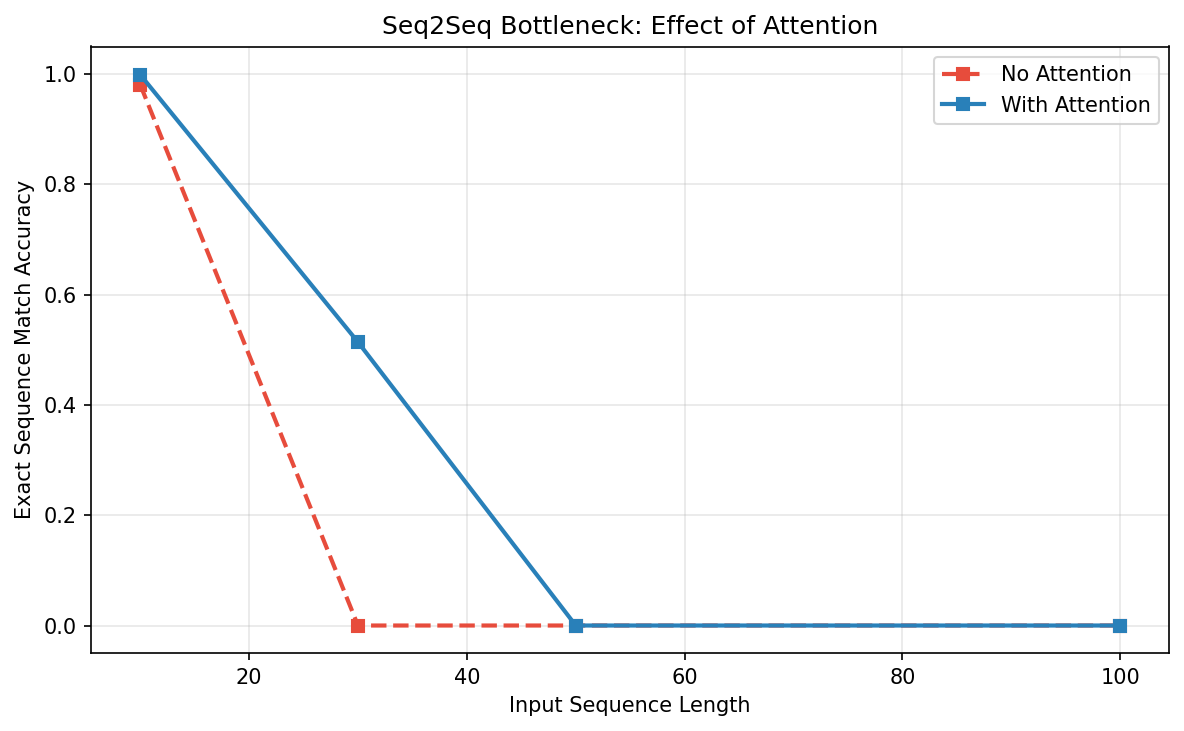
\includegraphics[width=0.6\textwidth]{labs/ch01/answers/figures/accuracy_vs_length.png}
\caption{Accuracy vs.\ input length. No-attention Seq2Seq collapses at length 30; attention extends usability.}
\label{fig:app-lab1-seq2seq}
\end{figure}

\begin{figure}[h]
\centering
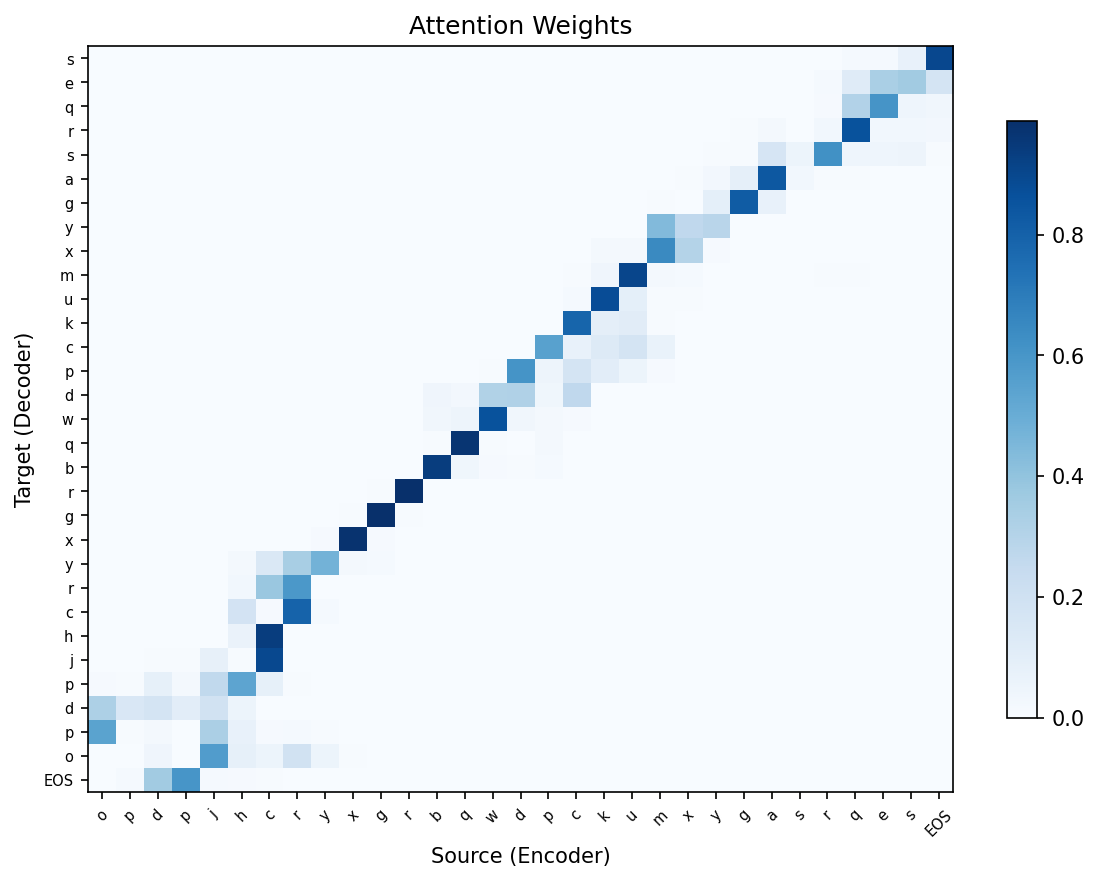
\includegraphics[width=0.55\textwidth]{labs/ch01/answers/figures/attention_heatmap.png}
\caption{Attention heatmap showing the expected anti-diagonal pattern for sequence reversal.}
\label{fig:app-lab1-attn}
\end{figure}

\textbf{Diagnosis:} The no-attention model succeeds at length 10 but collapses completely at length 30---the fixed encoder vector cannot store 30 position-specific details. Attention extends the usable range by allowing the decoder to read from all encoder states. The length-50/100 failures reflect training budget limitations, not a fundamental mechanism failure (the heatmap shows correct anti-diagonal alignment at the working lengths).

\textbf{Core insight:} This experiment makes the \emph{information bottleneck} tangible. A fixed-size encoder vector of dimension $d$ offers a constant-size communication channel between encoder and decoder. For the reversal task, the decoder needs to recall the exact token at a specific source position---roughly $\log(V)$ bits per position. As input length grows, the demand grows with sequence length while the context vector size stays fixed, so the bottleneck becomes increasingly severe. Attention changes the communication pattern: the decoder can directly address any encoder position, so accessible information scales with input length rather than being capped by a single fixed vector.

\textbf{Connection to Ch2--3:} This bottleneck is the historical motivation for attention (Bahdanau et al., 2015). The Transformer (Ch2) takes this further---self-attention removes the serial encoder entirely, and the decoder-only GPT (Ch3) eliminates the encoder/decoder distinction altogether. But the core insight is the same: \emph{fixed-size state is the enemy of long-range computation}. Gates alleviate this for recurrent models; attention eliminates it entirely.

%----------------------------------------------------------------------
\section{Lab 1 Synthesis: The Problem Escalation}

The five experiments form a chain of escalating problems and solutions:

\begin{center}
\begin{tabular}{llll}
\toprule
\textbf{Problem} & \textbf{Exposed By} & \textbf{Solved By} & \textbf{But\ldots} \\
\midrule
Word sense collapse & Exp 0 & Contextual RNN & Sequential, slow \\
Gradient explosion & Exp 1 & LSTM/GRU gates & Still serial \\
Information loss over distance & Exp 2 & Cell state highway & Fixed-size state \\
--- & Exp 3 & GRU (efficient gates) & Still bottleneck \\
Seq2Seq information bottleneck & Exp 4 & Attention & Still recurrent \\
\bottomrule
\end{tabular}
\end{center}

Each solution in the rightmost column creates the starting condition for the next chapter's problem. Ch2 addresses the final ``But'': if attention removes the bottleneck, why keep recurrence at all? The answer is the Transformer.
